
%
%Author: In this template, the places where you need to add information
%        (or delete line) are indicated by {???}.  Mostly the information
%        required is obvious, but some explanations are given in lines starting
%Author:
%All other lines should be ignored.  After editing, there should be
%no instances of ??? after this line.

% use option [preprint] to remove info line at bottom
% journal options: aop,aap,aos,aoas,ssy
% natbib option: authoryear
\documentclass[aap,preprint]{imsart}

\usepackage{amsthm,amsmath,amssymb}
\usepackage[square,sort,comma,numbers]{natbib}
\usepackage{tikz,caption}
\usepackage{pgfplots}
\usepackage{subcaption}
\RequirePackage[colorlinks,citecolor=blue,urlcolor=blue]{hyperref}

% provide arXiv number if available:
%\arxiv{arXiv:0000.0000}

\startlocaldefs
\newtheorem{notation}{Notation}
\newtheorem{lemma}{Lemma}
\newtheorem{theorem}{Theorem}
\DeclareMathOperator{\E}{\mathbb{E}}
\DeclareMathOperator{\p}{\mathbb{P}}
\pgfplotsset{
    colormap={blackwhite}{[5pt]
        rgb255(0pt)=(255, 255, 0);
        rgb255(245pt)=(0, 0, 0);
        rgb255(255pt)=(0, 0, 255);
        rgb255(1000pt)=(200, 255, 255)
    },
}
\endlocaldefs

\begin{document}

\begin{frontmatter}

\title{An Engineered Empirical Burnstein Bound}
\runtitle{An Engineered Empirical Burnstein Bound}

\begin{aug}
\author{\fnms{Mark} \snm{Burgess}\corref{}\thanksref{t1}
\ead[label=e1]{mark.burgess@anu.edu.au}
\ead[label=e2]{markburgess1989@gmail.com}}
\thankstext{t1}{A great thanks to Archie Chapman, Paul Scott and Sylvie Thiebaux; for Academic advice and encouragement!}
\address{Mark Alexander Burgess\\College of Engineering \& Computer Science\\Australian National University\\Canberra, ACT, Australia, 2600\\\printead{e1}\\
\printead{e2}}
\affiliation{Australian National University}
\end{aug}

\runauthor{M. Burgess}

\begin{abstract}
We derive a stronger Empirical Burnstein Bound (EBB) using a combination of Chernoff bounds and probability unions.
Like other EBBs, our EBB is a concentration inequality for the divergence of the sample mean from the population mean in terms of the sample variance.
The new EBB is numerically solved and compared against previous work, and also against a bound with perfect information about the variance.
The analysis reveals that our technique can shrink existing probability bounds by about a third, and that perfect variance information would reduce it by about a third again.
\end{abstract}

\begin{keyword}[class=MSC]
\kwd[60E15]{}
\kwd[; 62H10]{}
\end{keyword}

\begin{keyword}
\kwd{Concentration inequality}
\kwd{Chernoff bounds}
\kwd{Hoeffdings inequality}
\kwd{Emperical Burnstein Bound}
\end{keyword}

\end{frontmatter}






\section{Introduction}

Sample statistics are sometimes used to estimate the statistical parameters of the population (eg. mean, variance, etc).
And different methods of doing this are available depending on the sample statistics provided and the assumptions which are made about the population.
A recent development is Empirical Burnstein Bounds (EBB)\cite{Maurer50empiricalbernstein,10.1007/978-3-540-75225-7_15} which are probability bounds describing the likely divergence of the sample mean from the mean in terms of the sample variance under assumption that the population data is bounded within an interval of a known width.
EBBs have been used as a method of giving confidence bounds for the mean, which is a common and important process in many industrial applications.
We take inspiration and extend Maurer and Pontil's work \cite{Maurer50empiricalbernstein} as we combine older techniques to develop a new and stronger EBB

\section{Related Work}
Concentration inequalities are particular probabilistic bounds describing how much a random variable is expected to deviate (or otherwise be concentrated) around a particular value.
Famous historical concentration inequalities have often describe the expected deviation of sample statistics.
For instance, Chebyshev's inequality was known as far back as 1853\cite{Chebyshev1}, and some of the early Burnstein inequalities were published in the 1920s \cite{burnstein1}.
Since then, various analysis has yielded a wide range new concentration inequalities\cite{MR3363542,Boucheron2004}; particularly important are the innovations concerning the concentration of more general functions of random variables - for instance the Effron-Stein\cite{efron1981} and Entropy methods \cite{Boucheron_concentrationinequalities}, and applications of Talagrand's concentration inequality\cite{Talagrand1995}.

Inequalities such as these can describe the expected deviation of sample statistics - particularly often the sample mean, such as famously the Burnstein's inequalities \cite{burnstein1}, Hoeffding's inequalities \cite{hoeffding1} Bennett's inequalities \cite{10.2307/2282438} among others.
These inequalities have been used in various contexts, such as in machine learning and hypothesis testing.\cite{Maron1997,Mnih:2008:EBS:1390156.1390241,8000571,Zia-UrRehman2012,DBLP:conf/aaai/ThomasTG15,Maurer50empiricalbernstein}
Recently, the sample variance has also been incorporated into this process as EBBs \cite{Maurer50empiricalbernstein,10.1007/978-3-540-75225-7_15} and it remains to be seen how much these EBBs can be sharpened.

\section{Structure}

\begin{itemize}{\leftmargin=1em}
\item[-] We begin in section \ref{background} with fundamental concepts: probability unions, Chernoff bounds, and a decomposition of the sample variance into the mean of sample squares and sample mean.
\item[-] In section \ref{derivation} we outlay two Chernoff bounds (for the sample mean and the mean of sample squares) and use them with a probability union and variance decomposition to create a novel probability bound for the sample variance. After this we use probability union again to create a new EBB.
\item[-] In section \ref{evaluation} we numerically evaluate our EBB and compare it against Maurer and Pontil's EBB to show improvements.
\item[-] In section \ref{discussion} we give some simple expressions as envelopes over our numerical EBB and finish with a caution about its use.
\end{itemize}

\section{Background}\label{background}

To begin we introduce useful lemmas that form the basis for our derivation, the first is an often used result related to union bounds:

\begin{lemma}[Probability Union]\label{prob_union}
For random variables $a,b,c$ that:\\ $\p(a>c) \le \p(a>b) + \p(b>c)$
\end{lemma}
\begin{proof}
For any events $A$ and $B$ that:\\
$\p(A\cup B)\le \p(A)+\p(B)$
hence:\\
$\p((a>b) \cup (b>c))\le \p(a>b) + \p(b>c)$\\
If $a>c$ then $(a>b) \cup (b>c)$ is true irrespective of $b$ hence:\\
$\p(a>c) \le \p((a>b) \cup (b>c))$ and the conclusion follows.
\end{proof}

If $\p(a>c)$ is unknown but if a relationship between $a$ and some $b$, and also between $b$ and $c$ is known, then such a probability union may be useful.
The next lemma is a quick and well known result that relates the value of the sample mean and the value of sample squares to the sample variance.

\begin{lemma}[Variance Decomposition]\label{variance1}
For $\hat{\sigma}^2$ as sample variance, $\hat{\sigma}_0^2$ as average of sample squares, and $\hat{\mu}$ as sample mean, then:
$ \hat{\sigma}_0^2 = \hat{\mu}^2+\frac{n-1}{n}\hat{\sigma}^2 $
\end{lemma}
\begin{proof}
for samples $x_i$ that\\
$\hat{\sigma}^2=\frac{1}{n-1}\sum_i(x_i-\frac{1}{n}\sum_jx_j)^2 = \frac{1}{n-1}\sum_i(x_i-\frac{1}{n}\sum_jx_j)^2$\\
$=\frac{1}{n-1}(\sum_ix_i^2-\frac{1}{n}\sum_i\sum_jx_ix_j) = \frac{1}{n-1}(n\hat{\sigma}_0^2-n\hat{\mu}^2)$.
\end{proof}

It is by this equality that we will create bounds for the sample variance from bounds on the sample squares and sample mean.
However, In order to get these bounds we will use the next lemma. This lemma is the basis of a large number of inequalities called Chernoff bounds and is an application of Markov's inequality to give bounds on the mean of random variables\cite{hoeffding2}:

\begin{lemma}[Chernoff Bound]\label{chernoff1}
If $\hat{\mu}$ is sample mean of $n$ samples of random variable $X$ then for any $s>0$ and $t$:
$$ \textstyle\p(\hat{\mu}\ge t)\le\frac{\E\left[\exp(sX)\right]^n}{\exp(snt)} $$
\end{lemma}
\begin{proof}
$\p(\hat{\mu}\ge t) = \p(\exp(s\sum_ix_i)\ge \exp(snt))$\\
$\p(\hat{\mu}\ge t) \le \E[\exp(s\sum_ix_i)]\exp(-snt)$ via Markov's inequality \\ 
$\p(\hat{\mu}\ge t) \le \E\left[\exp(sX)\right]^n\exp(-snt)$ assuming i.i.d of samples.
\end{proof}

We will be using this to get the bounds on the sample mean and the mean of sample squares.
And with lemmas \ref{prob_union} and \ref{variance1} we will create a new EBB.

\section{Derivation}\label{derivation}

Our first probability bound is a Chernoff bound on the sample mean. This bound is not new and was derived by Wassily Hoeffding\footnote{Apparently it is also known as Bennet's inequality\cite{MR1782937}} \cite{hoeffding1} and has subsequently been a subject of discussion and many further developments \cite{hoeffding2,Bentkus08boundsfor,Pinelis2014,zbMATH00812598,MR1782937}.

\begin{theorem}[Hoeffding's inequality]\label{hoeffdings1}
For a random variable with a mean of zero that is bounded $a\le X\le b$, then the mean $\hat{\mu}$ of $n$ samples is probability bounded. For $t>0$:
\begin{equation}\label{eq_no2} \textstyle\p(\hat{\mu}\ge t)\le 
\left(\left(\frac{\sigma^2}{b^2}(\frac{\sigma^2}{b^2}+\frac{t}{b})^{-1}\right)^{\frac{\sigma^2}{b^2}+\frac{t}{b}}
\left(1-\frac{t}{b}\right)^{\frac{t}{b}-1}\right)^{n(\frac{\sigma^2}{b^2}+1)^{-1}} = H_1^n\left(\frac{\sigma^2}{b^2},\frac{t}{b}\right) \end{equation}
\end{theorem}
\begin{proof}
For $\alpha,\beta,\gamma$ that $\alpha s^2X^2+\beta sX+\gamma\ge \exp(sX)$ for all $a\le X\le b$:\\
$E\left[\exp(sX)\right] \le \E[\alpha s^2X^2+\beta sX+\gamma] = \alpha s^2\E[X^2]+\gamma = as^2\sigma^2+c$\\
If $c=\max(sa,sb)$ choosing $\alpha,\beta,\gamma$ to minimize the expression leads\footnote{see Appendix \ref{appendix1}} to:\\
$E\left[\exp(sX)\right] \le (s^2\sigma^2\exp(c) + c^2\exp(-s^2\sigma^2/c))/(s^2\sigma^2 + c^2) $\\
Hence by application of our lemma \ref{chernoff1}:\\
$ \textstyle\p(\hat{\mu}\ge t)\le \left(s^2\sigma^2\exp(c) + c^2\exp(-s^2\sigma^2/c)\right)^n\exp(-nst)(s^2\sigma^2 + c^2)^{-n} $\\
minimizing with respect to $s$ gives the result.
\end{proof}
We will also use a double sided version:
\begin{equation}\label{eq_no1} \textstyle\p(|\hat{\mu}|\ge |r|)=\p(\hat{\mu}^2\ge r^2)\le H_1^n\left(\frac{\sigma^2}{b^2},\frac{r}{b}\right)+H_1^n\left(\frac{\sigma^2}{a^2},\frac{-r}{a}\right) \end{equation}
The assumption that the mean is zero occurs without a loss of generality.
And in this way Hoeffding's inequality gives us a probability bound for the divergence of the sample mean from the true mean given the variance. However in practice we often don't know the variance but can only estimate it via a sample variance statistic.
So we endeavor to create a bound to characterize the divergence of the sample variance from the variance, we begin with a bound on the sample squares:


\begin{lemma}[Sample Square bound]\label{sample_squares}
For a random variable with a mean of zero that is bounded $a\le X\le b$, then the mean $\hat{\sigma}_0^2$ of $n$ samples squares is probability bounded:
\begin{align*} \p(\sigma^2 - \hat{\sigma}_0^2> y) \le \min_{\substack{s>0,\alpha,\beta,\gamma \\ \text{s.t}~\alpha x^2 + \beta x + \gamma\ge\exp(-sx^2)\\ \forall x\in[a,b]}} &\left(\exp(s(\sigma^2-y))(\alpha\sigma^2 + \gamma)\right)^n \\& ~~= H_2^n(a,b,y,\sigma^2)
\end{align*}
\end{lemma}
\begin{proof}
For $\alpha,\beta,\gamma$ that $\alpha X^2 + \beta X + \gamma \ge \exp(-qX^2)$ for all $a\le X\le b$:\\
$ \E[\exp(-qX^2)] \le \E[\alpha x^2 +\beta x +\gamma] \le \alpha\sigma^2 + \gamma $\\
Applying lemma \ref{chernoff1} to the mean of minus sample squares, gives:\\
$\p(-\hat{\sigma}_0^2\ge t) \le (\alpha\sigma^2 + \gamma)^n\exp(-snt) $\\
Substituting $t$ for $y-\sigma^2$ gives:\\
$\p(\sigma^2 - \hat{\sigma}_0^2> y) \le ((\alpha\sigma^2 + \gamma)\exp(s(\sigma^2-y)))^n $\\
Minimizing subject to constraints gives result.
\end{proof}

This probability bound is not easily put into closed form and so we will use numerics to evaluate it as necessary.
It is worth noting that the domain of function $H_2^n$ is restricted, firstly that it is defined for $a<0<b$ and secondly that $\sigma^2\le-ab\le (b-a)^2/4$ per Popoviciu's inequality \cite{zbMATH05780164}. It is important that these restrictions should propagate with the analysis.

At this point we have a probability bound on the mean squared by equation \ref{eq_no1} and also a probability bound on the sample squares by lemma \ref{sample_squares}. We proceed by using lemma \ref{variance1} to create a bound on the sample variance as follows:

\begin{theorem}[Sample Variance Bound]\label{variance2}
For a random variable that is bounded $a\le X\le b$ with variance $\sigma^2$ and a mean of zero, the sample variance $\hat{\sigma}^2$ of $n$ samples is probability bounded:
\begin{align}\label{eq_no8} \p(\sigma^2 - \hat{\sigma}^2 > w)\le &\min_{\phi\in[0,1]}
\begin{pmatrix}
	H_2^n\left(a,b,(1-\phi)(\frac{n-1}{n}w+\frac{1}{n}\sigma^2),\sigma^2\right)\\
	+H_1^n\left(\frac{\sigma^2}{b^2},\frac{\sqrt{\phi(\frac{n-1}{n}w+\frac{1}{n}\sigma^2)}}{b}\right)\quad\quad\\
	+H_1^n\left(\frac{\sigma^2}{a^2},\frac{-\sqrt{\phi(\frac{n-1}{n}w+\frac{1}{n}\sigma^2)}}{a}\right)
\end{pmatrix} \\
&=H_3^n(a,b,w,\sigma^2)\nonumber\end{align}
\end{theorem}
\begin{proof}
By lemma \ref{sample_squares}: $\p(\sigma^2 - \hat{\sigma}_0^2> y) \le H_2^n(a,b,y,\sigma^2)$\\
So by lemma \ref{variance1}: $\p\left(\sigma^2 - \hat{\sigma}^2 > \frac{n}{n-1}\left(\hat{\mu}^2+y-\frac{1}{n}\sigma^2\right)\right) \le H_2^n(a,b,y,\sigma^2)$\\
Also by manipulatin the inner inequality of equation \ref{eq_no1}: \\$\p\left(\frac{n}{n-1}\left(\hat{\mu}^2+y-\frac{1}{n}\sigma^2\right)\ge \frac{n}{n-1}\left(r^2+y-\frac{1}{n}\sigma^2\right)\right)\le H_1^n\left(\frac{\sigma^2}{b^2},\frac{r}{b}\right)+H_1^n\left(\frac{\sigma^2}{a^2},\frac{-r}{a}\right)$\\
Applying union bound (lemma \ref{prob_union}) to the above two equations gives:\\
$\p\left(\sigma^2 - \hat{\sigma}^2 > \frac{n}{n-1}\left(r^2+y-\frac{1}{n}\sigma^2\right)\right) \le H_2^n(a,b,y,\sigma^2)+H_1^n\left(\frac{\sigma^2}{b^2},\frac{r}{b}\right)+H_1^n\left(\frac{\sigma^2}{a^2},\frac{-r}{a}\right)$\\
We let $w=\frac{n}{n-1}\left(r^2+y-\frac{1}{n}\sigma^2\right)$. And for a given $w$ we have a range of possible $r>0$ and $y>0$ which we want to parameterize over with $0\le\phi\le 1$:\\
$y(\phi) = (1-\phi)\left(\frac{n-1}{n}w+\frac{1}{n}\sigma^2\right)$ and
$r(\phi)^2 = \phi\left(\frac{n-1}{n}w+\frac{1}{n}\sigma^2\right)$\\
$\p\left(\sigma^2 - \hat{\sigma}^2 > w\right) \le H_2^n(a,b,y(\phi),\sigma^2)+H_1^n\left(\frac{\sigma^2}{b^2},\frac{r(\phi)}{b}\right)+H_1^n\left(\frac{\sigma^2}{a^2},\frac{-r(\phi)}{a}\right)$\\
The result follows by minimizing over $\phi$.
\end{proof}
This function $H_3^n$ is subject to similar restrictions as $H_2^n$.\\
Thus we now have a probability bound for the divergence of the sample variance from the variance, and by theorem \ref{hoeffdings1} we have a bound for the sample mean given the variance. We combine these two together to create a bound for the sample mean given the sample variance - and thus a new Empirical Burnstein Bound.
To proceed further we outlay a theorem that embodies a process slightly improved from that followed by Maurer and Pontil \cite{Maurer50empiricalbernstein}. We state some notation to ease the presentation:

\begin{notation}
For a function $f$ with numbered inputs, we denote the inverse of $f$ with respect to its $i$'th input (counting from one) as $f^{-i}$, assuming it exists.
\end{notation}

\begin{theorem}[Essential EBB]\label{ebb1} If we have bounds between the mean and sample mean, and the variance and sample variance:
\\ $\p(\hat{\mu}-\mu>t)\le h(\sigma^2,t)$\\
$\p(\sigma^2-\hat{\sigma}^2>w)\le f(\sigma^2,w)$ \\ 
for $f$ and $h$ depending on those two parameters (not exclusively)\\
if $z(\sigma^2,w) = \sigma^2-f^{-2}(\sigma^2,w)$ and $f^{-2}$ exists\\
if $z^{-1}$ exists and is monotonic increasing in its first argument\\
if $h^{-2}$ exists and is monotonically increasing in its first argument\\then for $x\in[0,y]$:\\
$\p(\hat{\mu}-\mu>h^{-2}(z^{-1}(\hat{\sigma}^2,y-x),x))\le y$
\end{theorem}
\begin{proof}
Substituting $w\rightarrow f^{-2}(\sigma^2,w)$ gives\\ 
$\p(\sigma^2-\hat{\sigma}^2>f^{-2}(\sigma^2,w))\le w$\\
thus:
$\p(z(\sigma^2,w)>\hat{\sigma}^2)\le w$\\
hence:
$\p(\sigma^2>z^{-1}(\hat{\sigma}^2,w))\le w$\\
so:
$\p(h^{-2}(\sigma^2,t)>h^{-2}(z^{-1}(\hat{\sigma}^2,w),t))\le w$

Substituting $t\rightarrow h^{-2}(\sigma^2,t)$ gives\\ $\p(\hat{\mu}-\mu>h^{-2}(\sigma^2,t))\le t$\\
applying probability union (lemma \ref{prob_union}) gives:\\
$\p(\hat{\mu}-\mu>h^{-2}(z^{-1}(\hat{\sigma}^2,w),t))\le t+w$\\
letting $y=t+w$ and $x=y-w$ gives:\\
$\p(\hat{\mu}-\mu>h^{-2}(z^{-1}(\hat{\sigma}^2,y-x),x))\le y$
\end{proof}

The result of this theorem is an EBB - that is a probabilistic bound for the divergence of the sample mean from the mean parametrized by the sample variance. Care must be taken in applying this theorem that all the assumptions hold, the inverses exist, and the domains of the functions are propagated through the analysis\footnote{see notes in Appendix \ref{appendix2}}.

In applying theorem \ref{ebb1} to the results of theorems \ref{variance2} and \ref{hoeffdings1} (letting $h(\sigma^2,t)=H_1^n\left(\sigma^2/b^2,t/b\right)$ and $f(\sigma^2,w)=H_3^n(a,b,w,\sigma^2)$) we typically don't know the values of $a$ and $b$ but instead know the mean is somewhere within a finite interval of width $D=b-a$.
So after applying theorem \ref{ebb1} we take the worst case values of $a$ and $b$ consistent with a given $D$ and $\sigma^2$, and take the best $x\in[0,y]$ subject to all other bounds.
And we are done.

\begin{figure}[h]
\centering
\captionsetup{justification=centering,margin=0.01cm}
\begin{tikzpicture}
\begin{axis}[
	xmin=0,   xmax=0.25,
	ymin=0,   ymax=0.25,
	zmin=-0.15,   zmax=1.0,
	xtick={0.05,0.10,0.15,0.20,0.25},
	ytick={0.05,0.10,0.15,0.20},
	%ztick={-0.2,-0.1,0,0.1},
	xlabel=$\frac{\sigma^2}{D^2}$,
	ylabel=$\frac{w}{D^2}$,
	%zlabel=$blah$,
	xticklabel style={/pgf/number format/fixed},
	yticklabel style={/pgf/number format/fixed},
	zticklabel style={/pgf/number format/fixed},
	view={-110}{35},
	%point meta min=-0.3, point meta max=0.3,
	point meta min=-0.1, point meta max=0.3,
	title={Advantage over Entropic bound for n=200},
	%colorbar horizontal,
	colorbar,
	colorbar style={
        at={(1.07,0.66)},
		title=Advantage,
		%ylabel=Z-value,
		%ytick={-1,-0.75,...,1},
        height=0.54*\pgfkeysvalueof{/pgfplots/parent axis height},
		xticklabel style={
			text width=2.5em,
			%align=below,
			%anchor=north west,
			/pgf/number format/.cd,
			fixed,
			fixed zerofill
		}
	}
]
\addplot3[patch, shader=flat] 
	file
	{graph1.dat};
\end{axis}
\end{tikzpicture}
\caption{Our variance bound over Entropic bound:\\$\scriptstyle\exp\left(\frac{-(n-1)w^2}{2\sigma^2D^2}\right)-\max_{b\in\left[0.5,0.5-\sqrt{0.25-\sigma^2/D^2}\right]}H_3^n\left(D(1-b),Db,w,\sigma^2\right)$}
\label{biggraph2}
\end{figure}


\section{Evaluation}\label{evaluation}
Evaluating this new EBB consisted of numerically solving a minimization over a maximization over inversions of nested function minimizations.
This process was conducted in C and Python, using techniques of direct parameter searching, coordinate transforming of data points (for inversions) and interpolations as necessary.\footnote{see Appendix \ref{appendix2} for discussion of the details}
And through this process we were able to witness that the assumptions necessary for our theorems held true and thus were able evaluate our new EBB.

We began by comparing our variance bound (per theorem \ref{variance2}) against the entropic bound utilized in Maurer and Pontil's work \cite{Maurer50empiricalbernstein}, originally per \cite{MR2245497}:
\begin{equation}\label{eq:fe} \p(\sigma^2 - \hat{\sigma}^2>w) \le \exp\left(\frac{-(n-1)w^2}{2\sigma^2D^2}\right) \end{equation}
The advantage of our variance bound is shown in figure \ref{biggraph2}.
From this graph we see large regions of advantage and hence we suspect our variance bound may be of independent interest.
It is possible to take the minima of several bounds, hence we used the minima of our variance bound and the entropic bound in the creation of our EBB for good measure.

We also compared our EBB directly with Maurer and Pontil's EBB\cite{Maurer50empiricalbernstein}:
$$ \p\left(\mu-\hat{\mu}>\sqrt{\frac{2\hat{\sigma}^2\log(2/y)}{n}}+\frac{7D\log(2/y)}{3(n-1)}\right)<y $$
We felt were able to fairly compare in the domain of their EBB if had they carried Popoviciu's inequality in their derivation, specifically the domain where:
$$ \frac{1}{2}>\frac{\sqrt{\hat{\sigma}^2}}{D}+\sqrt{\frac{2\log(2/y)}{n-1}} $$
Hence we were able to plot the improvement our EBB offers in this domain, as shown in figure \ref{biggraph3}. In this graph a probability 0.5 bound is shown to approximately shrink by at least a third irrespective of $n$.
More generally we note that our expectations were confirmed as our refinement of their EBB was seen to be tighter across a large range of values.

We also compared the loss in confidence that our EBB gave over a bound which could be achieved with perfect information about the variance. Specifically Hoeffding's inequality\footnote{Hoeffding's inequality per theorem \ref{hoeffdings1} is understood here to be relatively tight.} assuming $\hat{\sigma}^2=\sigma^2$. The decrease of the bounds that perfect variance information would offer over our EBB is plotted in figure \ref{biggraph4}.
From this graph we notice that when the variance is small there is the most potential gain to be made and where uncertainty about the variance is most detrimental, but generally that going from our EBB to perfect variance information shrinks the bounds by about another third.

\begin{figure}[]
	\centering
    \begin{subfigure}[b]{.76\linewidth}
        \centering
		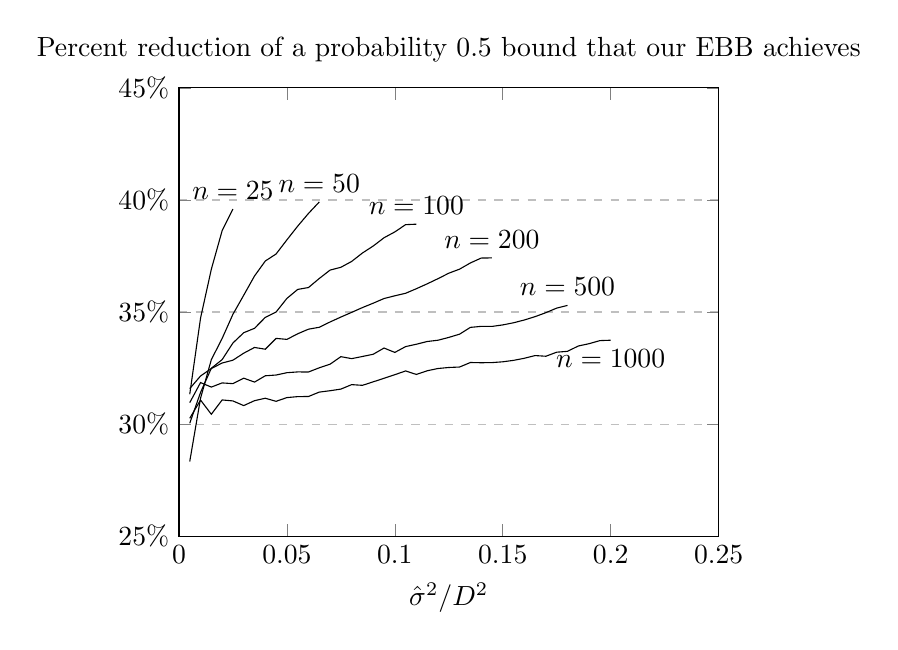
\begin{tikzpicture}
		\begin{axis}[
			title={Percent reduction of a probability 0.5 bound that our EBB achieves},
			xlabel={$\hat{\sigma}^2/D^2$},
			xmin=0, xmax=0.25,
			ymin=25, ymax=45,
			xtick={0,0.05,0.1,0.15,0.2,0.25},
			ytick={25,30,35,40,45},
			yticklabel=$\pgfmathprintnumber{\tick}\%$,
			ymajorgrids=true,
			grid style=dashed,
			xticklabel style={/pgf/number format/fixed},
		]
		\addplot[] coordinates {
		(0.005, 31.33262397944378)(0.01, 34.72886250674945)(0.015, 36.909296945183726)(0.02, 38.627583846687266)(0.025, 39.59462124039761)
			}node[pos=1.0](endofplotsquare){} ;
		\node [above] at (endofplotsquare) {$n=25$};
		\addplot[] coordinates {
		(0.005, 28.333532153239666)(0.01, 31.153830409409)(0.015, 32.87549096079947)(0.02, 33.81992265562242)(0.025, 34.89945361309619)(0.03, 35.74891595008532)(0.035, 36.60739883058407)(0.04, 37.276099921865196)(0.045, 37.59026746494855)(0.05, 38.218754538940686)(0.055, 38.83065159779602)(0.06, 39.39861647873854)(0.065, 39.910212250065214)
			}node[pos=1.0](endofplotsquare){} ;
		\node [above] at (endofplotsquare) {$n=50$};
		\addplot[] coordinates {
		(0.005, 30.038701393161688)(0.01, 31.412520149627277)(0.015, 32.49171315420119)(0.02, 32.876510879893)(0.025, 33.61899806422779)(0.03, 34.07734163182933)(0.035, 34.27418933046886)(0.04, 34.76092837396386)(0.045, 35.00082505166452)(0.05, 35.60742157468709)(0.055, 36.00845546401498)(0.06, 36.09363022383078)(0.065, 36.49561598871189)(0.07, 36.871363860949025)(0.075, 36.995564126738095)(0.08, 37.25705721710657)(0.085, 37.63281018078307)(0.09, 37.94537201050319)(0.095, 38.313563615135976)(0.1, 38.57428091364722)(0.105, 38.898129385115695)(0.11, 38.919035439297076)
			}node[pos=1.0](endofplotsquare){} ;
		\node [above] at (endofplotsquare) {$n=100$};
		\addplot[] coordinates {
		(0.005, 31.585709637284875)(0.01, 32.14640200496432)(0.015, 32.480242185958275)(0.02, 32.72477439020389)(0.025, 32.85137640603805)(0.03, 33.164192395805884)(0.035, 33.41972794004208)(0.04, 33.34159833965975)(0.045, 33.824240924074424)(0.05, 33.77957868846732)(0.055, 34.028900979162536)(0.06, 34.23479104354531)(0.065, 34.320408892537166)(0.07, 34.556516165135605)(0.075, 34.775904883097695)(0.08, 34.98535349546355)(0.085, 35.19862669231675)(0.09, 35.3945988354474)(0.095, 35.601977507693036)(0.1, 35.72487858163208)(0.105, 35.83625307070917)(0.11, 36.04135799347741)(0.115, 36.25828614993272)(0.12, 36.48817284893286)(0.125, 36.73194354036559)(0.13, 36.91341720219515)(0.135, 37.18914713784862)(0.14, 37.407683615789495)(0.145, 37.415360037546876)
			}node[pos=1.0](endofplotsquare){} ;
		\node [above] at (endofplotsquare) {$n=200$};
		\addplot[] coordinates {
		(0.005, 30.95805680601551)(0.01, 31.852731472234087)(0.015, 31.65165353001502)(0.02, 31.838019953330228)(0.025, 31.80514856457896)(0.03, 32.049553438239556)(0.035, 31.874671808872318)(0.04, 32.15628114167258)(0.045, 32.18970870320976)(0.05, 32.29347571578702)(0.055, 32.328022832020885)(0.06, 32.32551565971646)(0.065, 32.51203709690735)(0.07, 32.671571263469616)(0.075, 33.00950294213178)(0.08, 32.921019505844626)(0.085, 33.017153308081845)(0.09, 33.11615572233624)(0.095, 33.393651317961485)(0.1, 33.19788472106813)(0.105, 33.458020247263455)(0.11, 33.5638596989855)(0.115, 33.685389159897156)(0.12, 33.74232351659747)(0.125, 33.86778330552732)(0.13, 34.01232127428546)(0.135, 34.31523066744031)(0.14, 34.360222768291344)(0.145, 34.35739937066466)(0.15, 34.42537992870109)(0.155, 34.52118296490931)(0.16, 34.64446824473269)(0.165, 34.79488974531291)(0.17, 34.972098710274665)(0.175, 35.1757460413815)(0.18, 35.294877117787664)
			}node[pos=1.0](endofplotsquare){} ;
		\node [above] at (endofplotsquare) {$n=500$};
		\addplot[] coordinates {
		(0.005, 30.260287580516597)(0.01, 31.072712082932913)(0.015, 30.438989170134068)(0.02, 31.07887032375107)(0.025, 31.03408484266436)(0.03, 30.826085689381884)(0.035, 31.046097650764082)(0.04, 31.154259509093446)(0.045, 31.016858116914054)(0.05, 31.183097869794107)(0.055, 31.225975525465564)(0.06, 31.23249090698877)(0.065, 31.428023434202135)(0.07, 31.489666903553392)(0.075, 31.56173735319704)(0.08, 31.761301359885042)(0.085, 31.729964289057005)(0.09, 31.886510772066785)(0.095, 32.04347363722421)(0.1, 32.20435818840492)(0.105, 32.371965761927385)(0.11, 32.21538679904917)(0.115, 32.38001692151431)(0.12, 32.48085273757601)(0.125, 32.525780745561875)(0.13, 32.54658216492318)(0.135, 32.74841841730962)(0.14, 32.73824299176051)(0.145, 32.744293569773916)(0.15, 32.7796880354745)(0.155, 32.844022563820616)(0.16, 32.936888670494405)(0.165, 33.05787673349303)(0.17, 33.027986659386485)(0.175, 33.20865432723783)(0.18, 33.246662344351044)(0.185, 33.484850761982344)(0.19, 33.58811058089041)(0.195, 33.72513316286922)(0.2, 33.74255294433519)
			}node[pos=1.0](endofplotsquare){} ;
		\node [below] at (endofplotsquare) {$n=1000$};
		\end{axis}
		\end{tikzpicture}
		\caption{The percent reduction of the 0.5 probability bound, that going from Maurer and Pontil's EBB to our EBB would achieve, for various $n$, in the domain valid for their EBB.}
		\label{biggraph3}
    \end{subfigure}\\
    \vspace{5mm}
    \begin{subfigure}[b]{.76\linewidth}
        \centering
		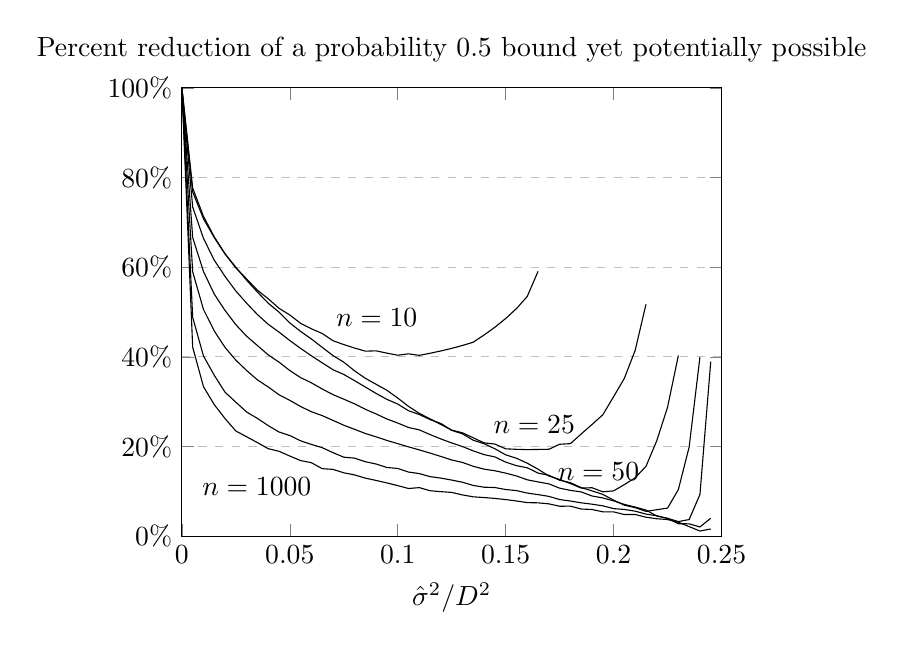
\begin{tikzpicture}
		\begin{axis}[
			title={Percent reduction of a probability 0.5 bound yet potentially possible},
			xlabel={$\hat{\sigma}^2/D^2$},
			xmin=0, xmax=0.25,
			ymin=0, ymax=100,
			xtick={0,0.05,0.1,0.15,0.2,0.25},
			ytick={0,20,40,60,80,100},
			yticklabel=$\pgfmathprintnumber{\tick}\%$,
			legend pos=south west,
			ymajorgrids=true,
			grid style=dashed,
			xticklabel style={/pgf/number format/fixed},
		]
		\addplot[] coordinates {
		(0.0, 100.0)(0.005, 76.80881648298994)(0.01, 70.80012751036021)(0.015, 66.60353535353535)(0.02, 62.960629921259844)(0.025, 59.830268741159834)(0.03, 57.38265464718681)(0.035, 54.86272684969753)(0.04, 52.966426490878426)(0.045, 50.833715771760744)(0.05, 49.34260238778903)(0.055, 47.48114630467571)(0.06, 46.261543044384865)(0.065, 45.21393912659903)(0.07, 43.60780860120358)(0.075, 42.741234424804404)(0.08, 41.970541970541966)(0.085, 41.27275292789615)(0.09, 41.34324249931186)(0.095, 40.828241683638836)(0.1, 40.36967586391642)(0.105, 40.67885117493473)(0.11, 40.33732457834427)(0.115, 40.80762478053674)(0.12, 41.318681318681314)(0.125, 41.896387832699624)(0.13, 42.54679916801479)(0.135, 43.2678270634475)(0.14, 44.87427466150871)(0.145, 46.60652040188641)(0.15, 48.55862874951305)(0.155, 50.767251676927316)(0.16, 53.47442378545112)(0.165, 59.068590983484604)
			}node[pos=0.7](endofplotsquare){} ;
		\node [above right] at (endofplotsquare) {$n=10$};
		\addplot[] coordinates {
		(0.0, 100.0)(0.005, 77.6561403508772)(0.01, 71.34845838015866)(0.015, 66.77283196861327)(0.02, 62.981189851268596)(0.025, 60.0)(0.03, 57.0902927514777)(0.035, 54.45127942244435)(0.04, 51.96859607876512)(0.045, 49.97258771929825)(0.05, 47.57404572092287)(0.055, 45.676705541500894)(0.06, 43.987817089452605)(0.065, 42.12854540723393)(0.07, 40.28687246647957)(0.075, 38.81136950904393)(0.08, 36.880072137060424)(0.085, 35.22028211023427)(0.09, 33.87552312037438)(0.095, 32.53546508941362)(0.1, 30.81437249047669)(0.105, 28.95112416489131)(0.11, 27.395132055929572)(0.115, 26.174496644295303)(0.12, 24.903425186711306)(0.125, 23.670007710100233)(0.13, 23.065173116089614)(0.135, 21.940071102082275)(0.14, 20.811153358681874)(0.145, 20.550688360450565)(0.15, 19.490254872563717)(0.155, 19.37869822485207)(0.16, 19.30933852140078)(0.165, 19.34787820666507)(0.17, 19.38534278959811)(0.175, 20.506329113924053)(0.18, 20.644283121597095)(0.185, 22.798605056669572)(0.19, 24.916247906197654)(0.195, 27.07537688442211)(0.2, 31.11861861861862)(0.205, 35.2304469273743)(0.21, 41.46645865834633)(0.215, 51.718869365928185)
			}node[pos=0.7](endofplotsquare){} ;
		\node [above right] at (endofplotsquare) {$n=25$};
		\addplot[] coordinates {
		(0.0, 100.0)(0.005, 73.41959943954505)(0.01, 66.4436173582515)(0.015, 61.55984585594049)(0.02, 57.93403164698015)(0.025, 54.687443245795656)(0.03, 51.969260326609025)(0.035, 49.440167949615116)(0.04, 47.26428079834825)(0.045, 45.52155103348822)(0.05, 43.63969363969365)(0.055, 41.895873454808815)(0.06, 40.23579989577905)(0.065, 38.6774968170317)(0.07, 37.13806461919406)(0.075, 36.073059360730596)(0.08, 34.695663042119726)(0.085, 33.263492802545294)(0.09, 31.835726416550862)(0.095, 30.517167250168896)(0.1, 29.4787827093551)(0.105, 27.9820525495266)(0.11, 27.141351798886053)(0.115, 25.998680422264876)(0.12, 25.14569457659372)(0.125, 23.599320882852297)(0.13, 22.825830083894598)(0.135, 21.39899438036083)(0.14, 20.631424375917767)(0.145, 19.502512341971507)(0.15, 18.148213342721355)(0.155, 17.384900322293685)(0.16, 16.283268301205524)(0.165, 14.950369495824049)(0.17, 13.428466886205634)(0.175, 12.641165755919854)(0.18, 11.73265528514348)(0.185, 10.732414793328498)(0.19, 10.808876163206872)(0.195, 9.896391568417291)(0.2, 10.109193377949982)(0.205, 11.514736120630568)(0.21, 13.028990336554482)(0.215, 15.574032619123763)(0.22, 21.29793510324484)(0.225, 28.771466314398943)(0.23, 40.30243261012492)
			}node[pos=0.745](endofplotsquare){} ;
		\node [above] at (endofplotsquare) {$n=50$};
		\addplot[] coordinates {
		(0.0, 100.0)(0.005, 66.63264504985476)(0.01, 59.04596954607779)(0.015, 53.999488883209814)(0.02, 50.347727640304065)(0.025, 47.17075223238636)(0.03, 44.61167971101746)(0.035, 42.5287356321839)(0.04, 40.44242768009076)(0.045, 38.82229464729603)(0.05, 36.95086234949561)(0.055, 35.37062155908402)(0.06, 34.21394768318686)(0.065, 32.83438879293802)(0.07, 31.577620967741936)(0.075, 30.56930693069307)(0.08, 29.513914294773297)(0.085, 28.306342780027)(0.09, 27.2679657647577)(0.095, 26.1414503133393)(0.1, 25.240174672489086)(0.105, 24.242424242424242)(0.11, 23.719661228897856)(0.115, 22.66414141414141)(0.12, 21.690588327422837)(0.125, 20.795378804710058)(0.13, 19.986774673499745)(0.135, 19.030112044817923)(0.14, 18.19329010922065)(0.145, 17.679088336256697)(0.15, 16.523420713364853)(0.155, 15.733937115516067)(0.16, 15.263202437373053)(0.165, 14.070096816471484)(0.17, 13.594470046082947)(0.175, 12.479061976549408)(0.18, 11.941848390446522)(0.185, 10.83476924993254)(0.19, 10.110966462091636)(0.195, 9.32322149863986)(0.2, 8.034350357128114)(0.205, 6.9143446852425186)(0.21, 6.365503080082135)(0.215, 5.532786885245901)(0.22, 5.906108026249369)(0.225, 6.26865671641791)(0.23, 10.4)(0.235, 19.900083263946712)(0.24, 39.94439295644115)
			}node[pos=1.0](endofplotsquare){} ;
		%\node [above] at (endofplotsquare) {$n=100$};
		\addplot[] coordinates {
		(0.0, 100.0)(0.005, 58.98664343786295)(0.01, 50.57766367137355)(0.015, 45.77709671715683)(0.02, 42.100909842845326)(0.025, 39.265978521530606)(0.03, 36.95646756871246)(0.035, 34.86590038314177)(0.04, 33.287324591672416)(0.045, 31.549749463135292)(0.05, 30.303030303030305)(0.055, 28.925445534113674)(0.06, 27.7629141798724)(0.065, 26.8988231513837)(0.07, 25.831202046035806)(0.075, 24.751099791618426)(0.08, 23.846328711070697)(0.085, 22.90933467404057)(0.09, 22.152617503755)(0.095, 21.356421356421354)(0.1, 20.641965664778876)(0.105, 19.924470242674317)(0.11, 19.246298788694478)(0.115, 18.532910658894913)(0.12, 17.784217265314382)(0.125, 17.0)(0.13, 16.44693473961766)(0.135, 15.58770225480432)(0.14, 14.952787478980731)(0.145, 14.591315453384416)(0.15, 14.068681753441997)(0.155, 13.438921122785)(0.16, 12.576495566379412)(0.165, 12.1045477014335)(0.17, 11.67240719479524)(0.175, 10.71428571428572)(0.18, 10.216812015503878)(0.185, 9.878838771593088)(0.19, 8.965888367365245)(0.195, 8.532969639468684)(0.2, 7.883082373782105)(0.205, 7.0957119967072035)(0.21, 6.501031561388886)(0.215, 5.830903790087479)(0.22, 4.503241633082184)(0.225, 3.994190268700073)(0.23, 3.258508327299059)(0.235, 3.7089871611982885)(0.24, 9.308510638297872)(0.245, 38.92587660896582)
			}node[pos=1.0](endofplotsquare){} ;
		%\node [above] at (endofplotsquare) {$n=200$};
		\addplot[] coordinates {
		(0.0, 100.0)(0.005, 48.82985928211302)(0.01, 40.20061728395061)(0.015, 35.8974358974359)(0.02, 32.10526315789474)(0.025, 29.89508775370134)(0.03, 27.697441601779754)(0.035, 26.26728110599078)(0.04, 24.66329966329966)(0.045, 23.238526179702653)(0.05, 22.453433091730965)(0.055, 21.28060263653484)(0.06, 20.47278564132497)(0.065, 19.744318181818187)(0.07, 18.640077551585644)(0.075, 17.621533663299214)(0.08, 17.415433403805487)(0.085, 16.612798965740136)(0.09, 16.096757852076994)(0.095, 15.320195510725066)(0.1, 15.115005476451262)(0.105, 14.304548450889918)(0.11, 13.963287073867834)(0.115, 13.283062645011604)(0.12, 12.956621004566218)(0.125, 12.517580872011253)(0.13, 12.032412032412036)(0.135, 11.314900744076228)(0.14, 10.927008880225257)(0.145, 10.857264866019005)(0.15, 10.408432147562582)(0.155, 10.170285892829247)(0.16, 9.61994026161294)(0.165, 9.276248725790005)(0.17, 8.879802110151953)(0.175, 8.181135851888914)(0.18, 7.840951319212183)(0.185, 7.4437788470980895)(0.19, 7.141815353201405)(0.195, 6.774544137181502)(0.2, 6.153993855606756)(0.205, 5.965045592705168)(0.21, 5.580409700965385)(0.215, 4.929577464788732)(0.22, 4.562383612662934)(0.225, 3.944315545243619)(0.23, 2.784222737819025)(0.235, 2.7586206896551726)(0.24, 2.059496567505721)(0.245, 4.0)
			}node[pos=1.0](endofplotsquare){} ;
		%\node [above] at (endofplotsquare) {$n=500$};
		\addplot[] coordinates {
		(0.0, 100.0)(0.005, 42.16746291174252)(0.01, 33.35416015828387)(0.015, 29.34782608695652)(0.02, 26.232905097389136)(0.025, 23.465482932802693)(0.03, 22.176210195630443)(0.035, 20.876445526475944)(0.04, 19.515807095486448)(0.045, 18.938835666912308)(0.05, 17.877821103627564)(0.055, 16.87069407276661)(0.06, 16.3916391639164)(0.065, 15.064102564102571)(0.07, 14.902449149024491)(0.075, 14.14141414141414)(0.08, 13.669774554782698)(0.085, 12.951474053768097)(0.09, 12.437623575934465)(0.095, 11.8800461361015)(0.1, 11.280101394169831)(0.105, 10.638865424798817)(0.11, 10.834674437823494)(0.115, 10.141206675224653)(0.12, 9.932659932659941)(0.125, 9.76821192052981)(0.13, 9.201954397394145)(0.135, 8.78038979304803)(0.14, 8.623417721518992)(0.145, 8.424908424908427)(0.15, 8.168754322600472)(0.155, 7.856817837099964)(0.16, 7.490636704119851)(0.165, 7.441688263606079)(0.17, 7.214611872146119)(0.175, 6.684027777777785)(0.18, 6.699077715021094)(0.185, 6.061680255228631)(0.19, 5.955012808365783)(0.195, 5.437352245862879)(0.2, 5.426783135016155)(0.205, 4.826880436636545)(0.21, 4.832613390928723)(0.215, 4.233870967741943)(0.22, 3.8909211839042195)(0.225, 3.712985556947849)(0.23, 3.1198686371100166)(0.235, 2.134646962233169)(0.24, 1.1494252873563218)(0.245, 1.6181229773462782)
			}node[pos=0.85](endofplotsquare){} ;
		\node [below left] at (endofplotsquare) {$n=1000$};
		\end{axis}
		\end{tikzpicture}
		\caption{The percent reduction in the 0.5 probability bound, that going from our EBB to Hoeffding's inequality (representing perfect knowledge of the variance, $\hat{\sigma}^2=\sigma^2$) achieves, for various n=10,25,50,100,200,500,1000.}
		\label{biggraph4}
    \end{subfigure}
\end{figure}


\section{Discussion}\label{discussion}
We also fitted some rough envelopes over our calculated numerics for $25\le n\le 1000$:
$$\scriptstyle \p\left(\sigma^2 - \hat{\sigma}^2>\frac{D^2}{\sqrt{n}}\left(0.09+0.3\log(1/w)+\frac{25w}{D^6}(\sigma^2)^2(D^2-4\sigma^2)+\frac{3}{2n}\right)\right) \le w$$
And
$$\scriptstyle \p\left(\mu - \hat{\mu}^2>\frac{D}{20\sqrt{n}}\left(16 - 10y + \frac{20D^2}{nD^2-4n\hat{\sigma}^2} + \left(y- \exp\left(-\frac{n^2}{16D^4}(1-4\hat{\sigma}^2)^2\right)\right)^{-1}\right)\right) \le y$$
\hfill When $\scriptstyle y-exp\left(-\frac{n^2}{16D^4}(1-4\hat{\sigma}^2)^2\right)>\frac{3}{20}$\\

Over our computed datapoints these envelopes were witnessed to always widen the probability bounds with a median width increase of $0.03367D^2$ across $7569$ datapoints and $0.0105D$ across $36918$ datapoints respectively.
These envelopes are supplied only as a loose approximation over the results of this paper and the reader is encouraged to explore the technique and source code\footnote{at: \href{https://github.com/Markopolo141/Engineered-Empirical-Burnstein-Bound}{https://github.com/Markopolo141/Engineered-Empirical-Burnstein-Bound}} if tighter or more accurate expressions are required.


 



\subsection{A Bayesian Caution}
The derivation of EBBs and similar bounds begin with population parameters (variance, mean, etc) and analytically bound the sample statistics relative to them (sample mean, sample variance, etc).
These bounds are thus implicitly statements of probability between sample statistics and population parameters, that are conditioned on those parameters.
However these can potentially be quite different from the same probability statements conditioned on the sample statistics.

I.e, if we know population parameters such as mean and variance we can analytically deduce probability bounds on sample mean and sample variance, however the converse process is potentially very different.

In various applications EBBs (and other similar bounds) have been used with sample statistics to give bounds on the population parameters. However it pays to note that this kind of use potentially goes beyond what can strictly be known by analysis.



\appendix

\section{Parabola Fitting}\label{appendix1}
For the task\footnote{Here we carry the derivation with the $x$-axis scaling factor $s$ removed for simplicity} of selecting an $\alpha,\beta,\gamma$ as the parameters of a parabola $\alpha x^2+\beta x+\gamma\ge \exp(x)$ for all $c\le x\le d$ which minimizes $z\alpha+\gamma$ for constants $c,d,z$.
We witness that any such parabola much tangentially touch the exponential curve at one point (at $x=f<d$) and intersect it at another (at $x=d$), as illustrated in the following figure \ref{fig:graph1}:
\begin{figure}[h]
\begin{tikzpicture}
\draw[->] (-3.5,0) -- (2,0) node[anchor=north] {$x$};
\draw[->] (0,0) -- (0,4) node[anchor=east] {};
\draw[smooth, domain=-3.5:2.0, color=black, line width=0.20mm] 
    plot (\x,{e^(\x)/2}) node [right] {\footnotesize $e^x$};
\draw[smooth, domain=-3.5:2.0, color=red, line width=0.20mm] 
    plot (\x,{(0.316137167001903*\x*\x + 1.39988395124422*\x + 1.67055451771745)/2}) node [right] {\footnotesize $\alpha x^2+\beta x+\gamma$};
\draw (1.5,-0.1) -- (1.5,{e^(1.5)/2});
\draw (-2,-0.1) -- (-2,{e^(-2)/2});
\draw (-2.5,-0.1) -- (-2.5,0);
\draw[black,fill] (1.5,{e^(1.5)/2}) circle (0.25mm);
\draw[black,fill] (-2,{e^(-2)/2}) circle (0.25mm);
\draw	(-2.5,-0.25) node{{\scriptsize $c$}}
		(-2,-0.25) node{{\scriptsize $f$}}
		(1.5,-0.25) node{{\scriptsize $d$}};
\end{tikzpicture}
\caption{\footnotesize Fitting a parabola above an exponential curve for all $c\le x\le d$}
\label{fig:graph1}
\end{figure}
The parabola's intersection at $x=d$ and its tangential intersection at $x=f$ can be written in matrix algebra:
$$
\begin{bmatrix}
    \alpha \\
    \beta \\
	\gamma
\end{bmatrix}
=
\begin{bmatrix}
    d^2 & d & 1 \\
    f^2 & f & 1 \\
	2f  & 1 & 0
\end{bmatrix}^{-1}
\begin{bmatrix}
    \exp(d) \\
    \exp(f) \\
	\exp(f)
\end{bmatrix}$$
which gives our parabola parameters $\alpha,\beta,\gamma$ in terms of $f$ and $d$, hence our objective function $z\alpha+\gamma$ can be written as:
$$z\alpha+\gamma = \frac{((z+fd-d)(f-d-1)-d)e^f+(f^2+z)e^d}{(d-f)^2}$$
since $d$ is fixed, minimizing with respect to $f$ gives $f=\frac{-z}{d}$ where our objective function becomes:
$$z\alpha+\gamma = \frac{ze^d + d^2e^{-z/d}}{z + d^2}$$
Which is sufficient for our purposes.

\section{Computational Process}\label{appendix2}
In this section we detail more closely the numerical approach we used to calculate our EBB.
We begin with the method used to numerically solve the function $ H_2^n(a,b,y,\sigma^2) $ per lemma \ref{sample_squares}.

\subsection{Computing $H_2^n(a,b,y,\sigma^2)$}
The function is a result of an optimization problem solving for the minima of an objective function subject to constraints: $$s>0,~\alpha,\beta,\gamma\quad  \text{s.t}~\alpha x^2 + \beta x + \gamma\ge\exp(-sx^2)\quad \forall x\in[a,b]$$
with $a<0<b$. Particularly this is over the family of parabolas fitting above an exponential $\exp(-sx^2)$ in the required range. Without loss of generality we consider $b>-a$ and also restrict the range of parabolas to thoes intersecting at $x=b$ and tangentially intersecting at another point $x=x_0$ as graphed in figure \ref{fig:graph2}. We note that the parabola characterized by $x_0=0$ is always valid, and that there exists a minimum value of $x_0$ such that all the parabolas $x_\text{min}\le x_0\le 0$ are all valid.
Analytically solving for $x_\text{min}$ is difficult, but it is simple enough that we can numerically determine it very quickly and accurately.

Then we take $n_1$ evenly spaced points of $x_0$ in the range $x_\text{min}\le x_0\le 0$, and $n_2$ evenly spaced points of $s$ in the range $0<s\le s_\text{max}$ and evaluate and take the minimum of the objective function for all combinations of these points. Note that any lack of resolution for these divisions (and/or unnecessary constriction in our choice of parabolas) would only serve to increase the computed value of $H_2^n(a,b,y,\sigma^2)$ which does not hamper the analytical accuracy of their use as an upper bound.


\begin{figure}
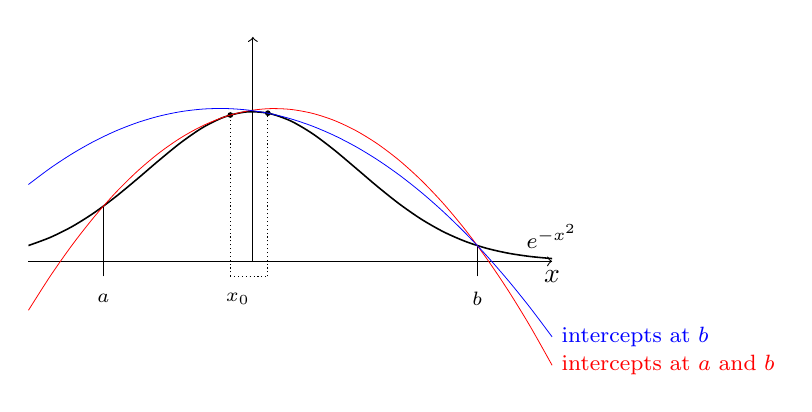
\begin{tikzpicture}[scale=1.9]
\draw[->] (-1.5,0) -- (2,0) node[anchor=north] {$x$};
\draw[->] (0,0) -- (0,1.5) node[anchor=east] {};
\draw[smooth, domain=-1.5:2.0, color=black, line width=0.20mm] 
    plot (\x,{e^(-\x*\x)}) node [above] {\footnotesize $e^{-x^2}$};
\draw (1.5,-0.1) -- (1.5,{e^(-1.5*1.5)});
\draw (-1,-0.1) -- (-1,{e^(-1*1)});

\draw[densely dotted] (-0.150534231,-0.1) -- (-0.150534231,{e^(-0.150534231*0.150534231)});
\draw[black,fill] (-0.150534231,{e^(-0.150534231*0.150534231)}) circle (0.15mm);
\draw[smooth, domain=-1.5:2.0, color=red, line width=0.10mm] 
    plot (\x,{(-0.49847785609681*\x*\x + 0.144246841020498*\x + 1.01060413924894)}) node [right] {\footnotesize intercepts at $a$ and $b$};

\draw[densely dotted] (0.1,-0.1) -- (0.1,{e^(-0.1*0.1)});
\draw[black,fill] (0.1,{e^(-0.1*0.1)}) circle (0.15mm);
\draw[smooth, domain=-1.5:2.0, color=blue, line width=0.10mm] 
    plot (\x,{(-0.30991666109058*\x*\x + -0.136026634531718*\x + 1.00675166381325)}) node [right] {\footnotesize intercepts at $b$};

\draw[densely dotted] (-0.150534231,-0.1) -- (0.1,-0.1);
\draw	(-0.1,-0.25) node{{\scriptsize $x_0$}}
		(-1,-0.25) node{{\scriptsize $a$}}
		(1.5,-0.25) node{{\scriptsize $b$}};
\end{tikzpicture}
\caption{\footnotesize parabolas above $\exp(-x^2)$ for all $a\le x\le b$, intercepting at $x=b$ and parametrized by a $x_0$ tangential intercept}
\label{fig:graph2}
\end{figure}


\subsection{Computing $H_3^n(a,b,w,\sigma^2)$}
The function is a result of an optimization problem solving for the minima of an objective function subject to constraint $\phi\in[0,1]$.
Straightforwardly this can be solved numerically by taking $n_3$ evenly spaced points of $\phi$ in the range $0\le\phi\le 1$ and taking the minimum of the objective function evaluated at each point.
Yet again, any lack of resolution for these divisions would only serve to increase the computed value of $H_3^n(a,b,w,\sigma^2)$ which does not hamper the analytical accuracy of its use as an upper bound. In this way the computed values of the variance bound of theorem \ref{variance2} should be analytically appropriate.

\subsection{Computing the EBB}
The next step in computing our EBB consisted in verifying assumptions and applying theorem \ref{ebb1}.
In the theorem \ref{ebb1} two interesting function inversions are necessary: $h^{-2}$ and $f^{-2}$.

The first is the inversion of Hoeffding's inequality on the second argument. Since Hoeffding's function is a closed form mathematical function and monotonically decreasing from $1$ to $0$ on the second argument, evaluating the inverse function at a point can be done quickly and accurately, furthermore the requirement that $h^{-2}$ be monotonically increasing in its first argument was not only witnessed numerically but also is intuitively recognized as being true of the function (that the increasing the variance would necessarily lead to widening probability bounds).

The second is the inversion of our computed function $H_3^n(a,b,w,\sigma^2)$ on its third argument - which is more difficult.
Generally, for any function, the values that the function takes can be plotted as points and the values that the inverse of that function takes can be determined by conducting coordinate swapping on those points. And so we evaluated $H_3^n(a,b,w,\sigma^2)$ across a range of input values and calculated $z^{-1}$ by coordinate swapping on those points. In this way $z^{-1}$ was witnessed to be a regular function monotonically increasing on its first argument.

After calculating datapoints for $z^{-1}$ we then made those datapoints regularly spaced by linear interpolation - at this point which it should be noted that specific analytical guarantees are lost as the process of interpolation can give datapoints that can be either below or above the underlying function.
In doing this interpolation we were thence able to appropriately compose the function as required by the theorem \ref{ebb1} as $h^{-2}(z^{-1}(\hat{\sigma}^2,y-x),x)$.
We did linear interpolation of $n_4$ data points evenly between $0$ and $1$ on the second argument.

We then took the maximum value of this bound for $a$ and $b$ consistent with a given $D=b-a$ and $\sigma^2$ specifically:
$$\max_{b\in\left[\frac{D}{2},\frac{D}{2}-\sqrt{\frac{D^2}{4}-\sigma^2}\right]} h^{-2}(z^{-1}(\hat{\sigma}^2,y-x),x)$$
We did this by taking $n_5$ evenly spaced values of $b$ in $\left[D/2,D\right]$ and considered those that satisfied $b<\frac{D}{2}-\sqrt{\frac{D^2}{4}-\sigma^2}$.
Then taking minimum $x$:
$$\min_{x\in[0,y]}\max_{b\in\left[\frac{D}{2},\frac{D}{2}-\sqrt{\frac{D^2}{4}-\sigma^2}\right]} h^{-2}(z^{-1}(\hat{\sigma}^2,y-x),x)$$
And in this context the values that have been computed for $x$ are implicitly constrained by the resolution of the interpolation $n_4$.

\subsection{Summary of Computation}
In this way we have detailed the components of the methodology used to evaluate our new EBB.
It is hoped that all of the components should be relatively transparent and simple numerical steps, and that the result of the method should be tunable without systematic bias to increasingly greater accuracy (at the cost of compute time) with parameters: $n_1,n_2,n_3,n_4,n_5$ and $s_\text{max}$.

For further information, the reader is encouraged to download, inspect and experiment with the sourcecode, available at:\\\href{https://github.com/Markopolo141/Engineered-Empirical-Burnstein-Bound}{https://github.com/Markopolo141/Engineered-Empirical-Burnstein-Bound}\\
The sourcecode consists of a small\footnote{$\sim 150$ lines of C code, and $\sim 250$ lines of Python code} documented package of C and Python code, that was used (and is setup) to compute the results of the paper.

\newpage
\bibliographystyle{imsart-number}
\bibliography{bib}


\end{document}
